\chapter{Bass-Serre-Theorie}

% =============
\section{Die Fundamentalgruppe eines Graphen}\label{sec_FG}

\DB Es sei $\GR$ ein zusammenhängender Graph und $p\in E(\GR)$.
\begin{enumerate}
\item $\pi_1(\GR,p)$ sei die Menge der stachelfreien geschlossenen
Wege in $\GR$ mit Anfangs- und Endpunkt $p$.
\item Für $w_1, w_2\in \pi_1(\GR,p)$ sei $w_1\cdot w_2$ der
Weg, den man nach dem Entfernen aller Stachel des aus $w_1$ und $w_2$
zusammengesetzen Weges erhält.
\item Mit dieser Verknüpfung ist $\pi_1(\GR,p)$ eine Gruppe.
Sie heißt \emph{Fundamentalgruppe}\index{Fundamentalgruppe}\index{Gruppe!Fundamental-}
von $\GR$ (bzgl. $p$).
\item Für jedes $q\in E(\GR)$ ist $\pi_1(\GR,q)\cong\pi_1(\GR,p)$.
Daher können wir auch $\pi_1(\GR)$ schreiben.
\end{enumerate}
\bew
\begin{itemize}
\item[3.] Das neutrale Element ist der Weg der Länge $0$.
Zu $w=(k_1,\ldots,k_n)$ ist
$\bar{w}=(\bar{k}_n,\ldots,\bar{k}_1)$ invers.

Die Zeichnung veranschaulicht, wie beim Zusammensetzen zweier
stachelfreier Wege neue Stachel autreten können.
\begin{center}
	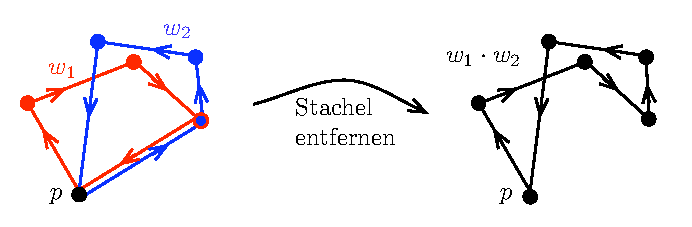
\includegraphics{w1w2}
\end{center}
Hat ein zusammengesetzter Weg $w=(k_1,\ldots,k_n)$ einen Stachel,
so muss $\bar{k}_i=k_{i+1}$ für ein $i$ gelten.
Setze $w^{(1)}:=(k_1,\ldots,k_{i-1},k_{i+2},\ldots,k_n)$ und
wiederholen dieses Vorgehen solange, bis alle Stacheln entfernt sind.
Wir bemerken, dass dies zu einem eindeutigen stachelfreien Weg führt.
Daraus folgt die Wohldefiniertheit der Verknüpfung und ebenso die
Assoziativität.
\item[4.] Es sei $v$ ein Weg in $\GR$ von $p$ nach $q$. Dann ist
\[
\phi:\pi_1(\GR,q)\Ra\pi_1(\GR,p),\quad
w\mapsto vw\bar{v}
\]
ein Gruppenhomorphismus, denn
\[
\phi(w_1 w_2) = v w_1 w_2 \bar{v}
=v w_1 \bar{v} v w_2 \bar{v}
=\phi(w_1)\phi(w_2).
\]
Da es offensichtlich eine Umkehrung gibt, ist $\phi$ bijektiv.
\qed
\end{itemize}

\BSP\
\begin{enumerate}
\item Ist $\GR$ ein Baum, so ist $\pi_1(\GR,p)=\{1\}$.
\item Es sei
\begin{center}
	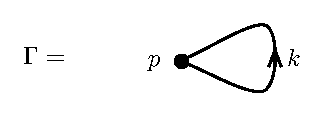
\includegraphics{pi1Z}
\end{center}
Die Gruppe $\pi_1(\GR,p)$ besteht aus dem Weg der Länge $0$
und aus den Wegen, die durch
$n$-faches Durchlaufen von $k$ oder $n$-faches Durchlaufen von
$\bar{k}$ entstehen. Daher ist $\pi_1(\GR,p)\cong\ZZ$.
\item Es sei
\begin{center}
	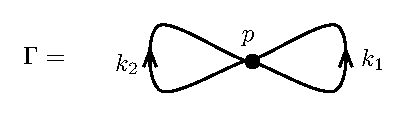
\includegraphics{pi1F2}
\end{center}
In diesem Fall ist $\pi_1(\GR,p)=F_2$.
\end{enumerate}

\PROP Für jeden zusammenhängende Graphen $\GR$ ist $\pi_1(\GR)$
eine freie Gruppe vom Rang $g(\GR)$.

\bew Für den Fall, dass $\GR$ hat nur eine Ecke hat:\\
...

Für den allgemeinen Fall:\\
Es sei $T$ ein aufspannender Teilbaum
von $\GR$ und $\GR':=\GR/T$. Nach Bemerkung \ref{bem_GZ}(2) ist
$g(\GR')=g(\GR)$. Zusammen mit dem Fall für eine Ecke genügt es
nun zu zeigen, dass $\pi_1(\GR')\cong\pi_1(\GR)$ ist.
\qed

\BEM Es sei $\GR$ ein zusammenhängender Graph und $Z$ ein Teilgraph.
Dann gibt es einen surjektiven Homomorphismus
$\phi_Z:\pi_1(\GR)\Ra\pi_1(\GR/Z)$ mit
$\K{\phi_Z}=\lag\pi_1(Z)\rag$.